% \section{Method}
% \label{sec:method}

% \begin{figure*}[t] 
% 	\centering
% 	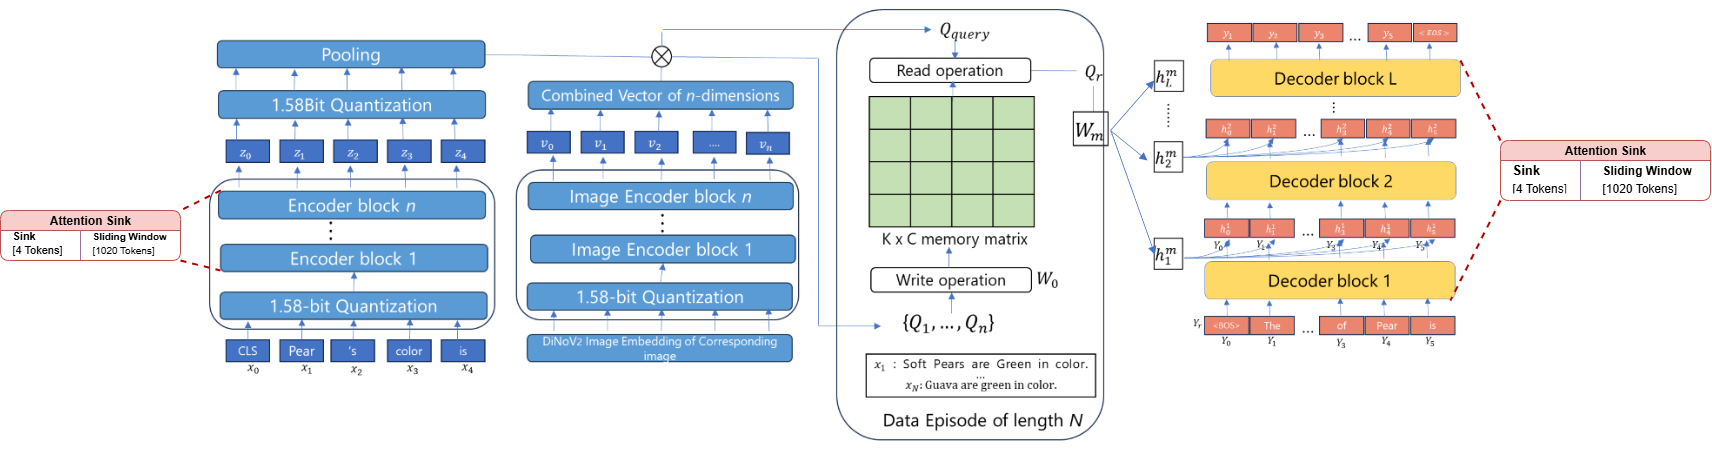
\includegraphics[width=\textwidth]{FIG/BitMar-Architecture.png}
% 	\caption{BitMar Architecture: $X$ and $X_{query}$ represent multimodal episode inputs - text tokens and corresponding DiNOv2-compressed image features. Quantized representations ($z$ and $v$) are computed via BitNet 1.58-bit quantized encoders for both text and vision branches, those encodings are pooled and fused into $Q$ and $Q_{query}$ using cross-modal attention. Attention sinks with a sliding window mechanism (4 sink tokens + 1020 window tokens) enable infinite context processing in both encoder and decoder blocks. A fixed-size $K \times C$ episodic memory matrix stores and retrieves cross-modal episode vectors with quantized read and write weights $(W, W_0)$, supporting SD card-based offloading for edge deployment.}
% 	\label{fig:bitmar}
% \end{figure*}

% We propose BitMar, a deployable, quantized multimodal language model designed for efficient image–text generation under resource constraints. The architecture follows a four-stage pipeline: (1) parallel low-bit encoders for text and vision inputs, (2) cross-modal fusion in a unified latent space, (3) context augmentation via an external episodic memory module, and (4) autoregressive decoding conditioned on both the fused representation and retrieved memory signals. The text encoder is a BitNet-based transformer operating at 1.58-bit precision, enabling compact yet expressive language representations. The vision encoder leverages a DiNOv2 backbone followed by quantization-aware compression to produce efficient visual embeddings. Cross-modal interaction is performed through a lightweight attention mechanism that aligns the 768-dimensional latent representations from both modalities. An external, fixed-size episodic memory stores multimodal context vectors from prior inputs and retrieves relevant entries during generation, injecting them into the decoder via per-layer conditioning. This memory-augmented decoder is inspired by Memory-Augmented Neural Networks (MANNs) introduced by~\citep{graves-dynamicexternalmemory-2016}, but diverges in its design by incorporating low-bit quantization and enabling cross-modal memory retrieval. While~\citep{graves-dynamicexternalmemory-2016} used a simple memory module for task-based memory storage and retrieval, BitMar's memory mechanism integrates both text and visual modalities to enhance multimodal generation, allowing for a richer representation of contextual information. The decoder itself is a BitNet-based autoregressive transformer equipped with streaming attention through attention sinks, allowing low-latency, long-context generation.

% \subsection{Text Encoders}
% \textbf{Architecture}. The text encoder is a lightweight, quantized Transformer designed to efficiently process language inputs under strict resource constraints. The architecture consists of four Transformer layers with a hidden dimension $d=128$ and four attention heads $h=4$, supporting sequences of up to 256 tokens. This compact configuration provides a balance between expressiveness and computational efficiency, making it suitable for deployment in low-latency environments.

% \textbf{Quantization}. To further reduce memory footprint and accelerate computation, we apply two levels of quantization:
% \begin{itemize}
%     \item \textbf{Weight Quantization}. All linear projection weights in the multi-head self-attention (MHSA) and feed-forward network (FFN) submodules are quantized to ternary values $\{-1,0,+1\}$ using learned per-layer scaling factors. This scheme corresponds to 1.58-bit quantization, where the scale parameter is trained jointly with the network parameters, allowing each layer to adapt its effective dynamic range.
%     \item \textbf{Activation Quantization}. Token-wise activations are quantized to 8 bits using per-token max-abs scaling. For each token embedding vector, we compute its maximum absolute value across dimensions and use it to scale the vector into the $[-127,127]$ integer range before discretization. This localized scaling preserves fine-grained detail for each token, mitigating the information loss often observed in global scaling methods.
% \end{itemize}

% This dual quantization strategy substantially reduces the model’s memory and compute requirements, while the combination of ultra-low-bit weights and 8-bit activations ensures stable training and inference.

% \textbf{Attention Sinks Injection}. To enable efficient processing of long or streaming sequences without quadratic growth in memory usage, we incorporate attention sinks into every self-attention layer. Let $S$ denote the number of sink tokens and $W$ the sliding-window size. During encoding, we maintain a key–value ($KV$) cache containing:

% \begin{itemize}
%     \item The first $S=4$ sink tokens, which are never evicted, serving as persistent global context anchors.
%     \item The most recent $W=1,020$ tokens, stored in a sliding window.
% \end{itemize}

% When a new token arrives, the cache evicts the oldest token in the window, merges the sink tokens with the updated window tokens, and clamps positional embeddings to the range $[0,S+W-1]$. This ensures that the model’s positional encoding space remains consistent despite the shifting window. The merged sink–window set is then used in the self-attention computation, enabling seamless attention over arbitrarily long contexts with fixed memory usage. This combination of low-bit quantization and streaming attention mechanisms allows the text encoder to operate effectively in constrained environments, maintaining high throughput while preserving long-range dependencies.

% \subsection{Vision Encoders}
% The vision encoder leverages pretrained DiNOv2 representations to provide high-quality visual features while avoiding the computational cost of full backbone inference during training and deployment. Specifically, 768-dimensional patch-level features are extracted offline for each image using a frozen DiNOv2 backbone~\citep{oquab-dinov2-2024}. This setup enables the model to operate without GPU-intensive convolutional or transformer vision stacks at inference time, reducing the overall system complexity.

% \textbf{Spatial Pooling}.
% Before compression, we apply 2×2 average pooling to the patch grid, reducing the total patch count by a factor of four. This operation decreases the token sequence length in subsequent processing while retaining coarse spatial structure. The pooled feature map maintains the same 768-dimensional embedding per patch.

% \textbf{Compression Module}.
% To align with the text encoder’s compact representation space and minimize memory footprint, we employ a learned two-layer MLP bottleneck to compress the 768-dimensional DiNOv2 features to a 128-dimensional latent vector. The transformation proceeds as:

% \vspace{-1.5em}
% \begin{align}
%     \mathbf{z}^{(1)}_{\text{vis}} &= \mathrm{ReLU}(\mathbf{W}_1 \mathbf{x}_{\text{vis}} + \mathbf{b}_1), \\
%     \mathbf{z}^{(2)}_{\text{vis}} &= \mathbf{W}_2 \mathbf{z}^{(1)}_{\text{vis}} + \mathbf{b}_2
% \end{align}
% \vspace{-1.5em}

% where $\mathbf{W}_1 \in \mathbb{R}^{384\times768}$, $\mathbf{W}_2 \in \mathbb{R}^{128\times384}$, and dropout is applied after the ReLU activation for regularization.

% \subsection{Cross-Modal Fusion}
% The cross-modal fusion module aligns and integrates the latent representations from the text and vision encoders into a unified multimodal representation. The module operates on pooled token embeddings from each modality: the text encoder output $ \mathbf{Z} \in \mathbb{R}^{n \times 128} $ and the vision encoder output $ \mathbf{V} \in \mathbb{R}^{n \times 128} $, where $n$ denotes the token length after pooling or spatial reduction.

% \textbf{Fusion Mechanism}.
% We adopt a standard cross-attention mechanism in which the text tokens act as the queries $(Q)$ and the vision tokens serve as the keys $(K)$ and values $(V)$. This design allows the text representation to selectively attend to relevant visual information, aligning semantic content in the text with spatial and object-level cues in the image features. The attention weights are computed as:

% \vspace{-1.5em}
% \begin{equation}
%     \mathrm{Attention}(Q, K, V) = 
%     \mathrm{softmax}\left( \frac{QK^\top}{\sqrt{d_k}} \right) V
% \end{equation}
% \vspace{-1.5em}

% where $d_k$ is the key dimensionality.

% \textbf{Quantization Strategy}.
% To maintain the model’s low-bit efficiency, all projection matrices used in generating $Q, K,V$ and the fused output are quantized to 1.58 bits using ternary weights $\{-1,0,+1\}$ with learned per-layer scaling factors. The softmax computation and the residual add–layer normalization operations are performed in FP32 to preserve numerical stability and avoid accumulation errors during attention score computation.

% The result of the cross-attention operation is the fused representation $ \mathbf{F} \in \mathbb{R}^{n \times 128} $ , where each text token embedding has been enriched with complementary visual information. To prepare this multimodal representation for interaction with the episodic memory module, we apply either mean pooling or a learned pooling operation over the sequence dimension to produce a single query matrix $ \mathbf{Q_{query}} \in \mathbb{R}^{n \times 128} $. This query matrix is subsequently used to retrieve relevant context vectors from the episodic memory, ensuring that the decoder is conditioned on both the current multimodal input and relevant prior experiences.

% \subsection{Episodic Memory}
% The episodic memory module augments the fused multimodal representation with contextual information stored across prior inference steps. The memory is implemented as a learnable matrix $ \mathbf{M} \in \mathbb{R}^{K \times C} $, with $K=512$ slots and embedding dimensionality $C=128$, where each slot stores a latent vector that summarizes the multimodal context from past inputs. After experimentation, we found that 512 memory slots provided a more effective capture of the latent space, resulting in improved contextual recall and memory utilization during decoding.

% \textbf{Writing}.
% At each generation step $ t \in [[1,n]] $, the current episodic query vector $ \mathbf{Q_{query,t}} \in \mathbb{R}^{C} $ is written into the memory via learned write weights $ \mathbf{W_{w}} \in \mathbb{R}^{K} $. The update rule is as follows:

% \vspace{-1em}
% \begin{equation}
% \mathbf{M} \leftarrow \mathbf{M} + \alpha \cdot \mathbf{W}w^\top \mathbf{Q}_{query,t}
% \end{equation}
% \vspace{-1.5em}

% where $\alpha=0.2$ is a fixed update rate controlling the influence of new entries. This formulation enables soft writing to multiple memory slots in proportion to $W_w$, rather than hard assignment to a single slot.

% \textbf{Reading}.
% To retrieve relevant context, we compute read weights using content-based addressing:

% \vspace{-1em}
% \begin{equation}
% \mathbf{W}r = \mathrm{softmax}(\mathbf{M} \mathbf{Q}_{query})
% \end{equation}
% \vspace{-1.5em}

% where the similarity between $Q_{query}$ and each memory slot determines its contribution. The retrieved memory vector is then:

% \vspace{-1em}
% \begin{equation}
% \mathbf{M}_r = \mathbf{W}_r^\top \mathbf{M} \in \mathbb{R}^{1 \times C}
% \end{equation}
% \vspace{-1.5em}

% which is concatenated or added to the fused multimodal representation before decoding.

% \textbf{External Storage}.
% For long-running sessions or deployment on memory-constrained devices, the memory matrix $M$ can be offloaded to external storage (e.g., an SD card) via a Python utility that saves and loads memory tensors without gradient tracking. This allows a persistent state between sessions without increasing runtime GPU memory usage.

% \textbf{Regularization}.
% To prevent drift and ensure stability, we apply an $\ell_2$ penalty to memory updates:

% \vspace{-1em}
% \[
% \mathcal{L}_{\text{mem}} = \lambda \|\Delta \mathbf{M}\|_2^2
% \]
% \vspace{-1.5em}

% Additionally, a usage-based forgetting mechanism gradually attenuates the contribution of slots that have not been accessed recently, ensuring that the memory remains relevant to the current context while preventing unbounded growth of stale information.


% \subsubsection{Decoder with Attention Sinks}
% The decoder is a lightweight, autoregressive transformer that generates text conditioned on both the current multimodal context and retrieved episodic memory signals. The architecture comprises four causal transformer layers, each with a hidden dimension of 128, four attention heads, and a maximum generation length of 256 tokens.

% \textbf{Attention Sinks for Long-Context Generation}.
% To support generation over sequences longer than the maximum length without quadratic growth in attention computation, we integrate attention sinks into every decoder self-attention layer. Each layer maintains a key–value $(KV)$ cache consisting of:~\textbf{Sink tokens}. The first $S$ tokens (persistent anchors) are never evicted, providing a stable global context.
% \textbf{Sliding window}. The most recent $W$ tokens that capture local dependencies.


% For each new token, the window cache evicts the oldest entry, merges with the sink tokens, and clamps positional indices to the range $[0, S + W - 1]$. This mechanism ensures consistent positional encoding and enables the decoder to attend to arbitrarily long contexts while keeping memory usage bounded.

% \textbf{Memory Integration}.
% At each decoding step, the retrieved memory vector $ \mathbf{M_{r}} \in \mathbb{R}^{1 \times 128} $ from the episodic memory module is projected through a learnable linear layer and then combined with the token input embeddings for the current step. The integration can be implemented in two ways:~\textbf{Concatenation}. $[x_{t}; M_{r}]$ is passed through a projection layer to match the decoder’s hidden size.
% \textbf{Addition}. $M_{r}$ is added directly to the input embedding $x_{t}$ as a residual conditioning signal. This conditioning allows the decoder to leverage both the current fused multimodal context and relevant episodic knowledge during text generation.

% \textbf{Output Projection}.
% The decoder’s final hidden states are mapped to vocabulary logits via a BitNet-quantized linear layer BitNetLinear (128 $\rightarrow$ 50,257), corresponding to the GPT-2 vocabulary size. While the projection weights are quantized for efficiency, the logits are computed in FP32 to preserve numerical stability in the subsequent softmax cross-entropy loss computation.

% \subsubsection{Training Objectives}
% The model is trained using a multi-objective loss function that combines generation, cross-modal alignment, and memory stability components.

% \textbf{Language Modeling Loss}.
% The primary objective is a language modeling loss $\mathcal{L}_{\text{lm}}$, implemented as the token-level cross-entropy between the decoder’s predicted probability distribution and the ground-truth caption tokens. At each decoding step $t$, the loss is:

% \vspace{-1.5em}
% \begin{equation}
% \mathcal{L}_{\text{lm}} = - \frac{1}{T} \sum_{t=1}^T \log p_{\theta}(y_t^\ast \mid y_{<t}, \mathbf{X})
% \end{equation}
% %\vspace{-1.5em}

% where $T$ is the target length, $y_t^\ast$ is the gold token at step $t$, and $X$ denotes the fused multimodal input. This term has a fixed weight of 1.0 in the total loss.

% \textbf{Cross-Modal Contrastive Loss}.
% To enforce alignment between modalities, we introduce a cross-modal contrastive loss $\mathcal{L}_{\text{cm}}$ following an InfoNCE formulation~\citep{oord_representation_2018}. Given a batch of paired text embeddings $z_{t}$ and vision embeddings $z_{v}$,  we compute cosine similarities for all pairs in the batch and apply a softmax over negative pairs:

% %\vspace{-1.5em}
% \small
% \begin{equation}
% \mathcal{L}{\text{cm}} = - \frac{1}{N} \sum_{i=1}^N \log \frac{\exp(\mathrm{sim}(\mathit{z}_t^i, \mathit{z}_v^i) / \tau)}{\sum{j=1}^N \exp(\mathrm{sim}(\mathit{z}_t^i, \mathit{z}_v^j) / \tau)}
% \end{equation}
% \normalsize
% %\vspace{-1.5em}

% where $\mathrm{sim}(\cdot, \cdot)$ denotes cosine similarity, $\tau$  is a temperature parameter, and $N$  is the batch size. This loss is applied symmetrically for both text-to-vision and vision-to-text retrieval and is weighted by 1.5.

% \textbf{Memory Consistency Loss}.
% To ensure stability in the episodic memory module, we introduce a memory consistency loss $\mathcal{L}_{\text{mem}}$, defined as the $\ell_2$ distance between consecutive memory write vectors:

% \vspace{-1.5em}
% \begin{equation}
% \mathcal{L}_{\text{mem}} = | \mathbf{M}^{(t)}_{\text{write}} - \mathbf{M}^{(t-1)}_{\text{write}} |_2^2
% \end{equation}
% %\vspace{-1.5em}

% This term discourages abrupt changes in stored memory representations and is weighted by 0.1.

% \textbf{Total Objective}.
% The final training objective is a weighted sum of the three components:

% %\vspace{-1.5em}
% \begin{equation}
% \mathcal{L} = \mathcal{L}_{\text{lm}} + 1.5 , \mathcal{L}_{\text{cm}} + 0.1 , \mathcal{L}_{\text{mem}}
% \end{equation}
% %\vspace{-1.5em}

% This formulation balances caption generation accuracy, cross-modal representation alignment, and stability in the episodic memory over time.

% \subsubsection{Adaptive Training Controller}
% To maintain stable multimodal alignment and mitigate the risk of modality collapse during training, we introduce an Adaptive Training Controller (ATC) that dynamically adjusts the optimization process based on online monitoring of cross-modal alignment metrics.

% \textbf{Monitoring Phase}.
% The ATC continuously tracks the exponential moving average (EMA) of the cross-modal cosine similarity between pooled text and vision embeddings. The EMA is computed over a rolling window of 200 training steps, providing a smoothed estimate of alignment trends while reducing the impact of short-term fluctuations.

% \textbf{Intervention Trigger}.
% An intervention is triggered if the EMA exhibits a relative drop greater than 0.12 compared to its recent maximum value and if at least 800 steps have elapsed since the last intervention. This dual criterion ensures that adjustments are applied only when there is a sustained and significant degradation in alignment, avoiding overreaction to minor noise.

% \textbf{Intervention Actions}.
% Upon triggering, the ATC randomly selects one of the following stabilization actions:
% \begin{itemize}
%     \item Freeze text encoder — temporarily halts updates to all parameters in the text encoder.
%     \item Freeze vision encoder — temporarily halts updates to all parameters in the vision encoder.
%     \item Boost cross-modal loss weight — increases the weight of the cross-modal contrastive loss $\mathcal{L}_{\text{cm}}$ to strengthen alignment learning.
% \end{itemize}

% The selected action is applied for a freeze duration of 1,500 training steps, during which the chosen component remains fixed or the loss weight remains boosted.

% \textbf{Stability Benefits}.
% By adaptively freezing one modality or emphasizing cross-modal supervision, the ATC prevents modality collapse, a failure mode where one encoder dominates the shared representation space, leading to degraded cross-modal retrieval and generation quality. This mechanism ensures that both encoders contribute meaningfully throughout training and that alignment remains stable even under challenging optimization conditions.

\section{Method}
\label{sec:method}

\begin{figure*}[t]
    \centering
    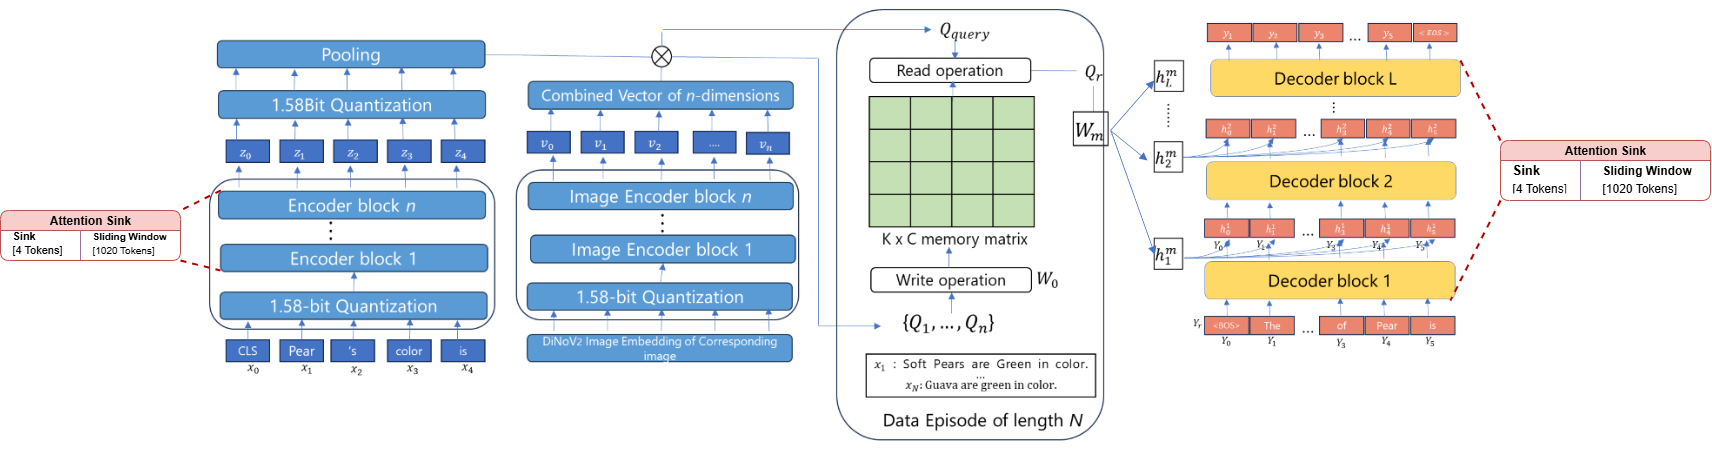
\includegraphics[width=\textwidth]{FIG/BitMar-Architecture.png}
    \caption{\textbf{BitMar Architecture.}
    The model processes multimodal inputs: text tokens and DiNOv2-compressed image features.
    Quantized encoders (1.58-bit) generate compact text and vision embeddings ($z$, $v$), which are fused via cross-modal attention into shared query representations ($Q$, $Q_{query}$).
    A sliding-window attention mechanism enables long-context processing.
    A fixed episodic memory matrix ($K \times C$) stores and retrieves multimodal context vectors through quantized read/write weights ($W$, $W_0$), supporting optional SD-card offloading for edge deployment.
    }
    % \caption{BitMar Architecture. $X$/$X_{query}$: multimodal inputs (text tokens + DiNOv2-compressed image features). Quantized encoders produce $z$/$v$ (1.58-bit). Cross-modal attention pools/fuses to $Q$/$Q_{query}$. Attention sinks with a sliding window (4 sink tokens, 1020 window) enable infinite-context processing. A fixed $K\times C$ episodic memory stores/retrieves episode vectors with quantized read/write weights $(W,W_0)$, supporting SD-card offloading.}
    \label{fig:bitmar}
\end{figure*}

We introduce \textbf{BitMar}, a deployable quantized multimodal LM for efficient image–text generation under tight resources. The four-stage pipeline is: 
(1) \textbf{parallel low-bit text/vision encoders}; 
(2) \textbf{cross-modal fusion} in a shared latent space; 
(3) \textbf{context augmentation} via external episodic memory; 
(4) \textbf{autoregressive decoding} conditioned on fused and retrieved signals. 
Text uses a BitNet transformer at 1.58-bit precision; vision uses DiNOv2 features plus quantization-aware compression. Fusion aligns 768-D modality latents via lightweight attention. A fixed-size episodic memory stores prior multimodal contexts and injects retrieved vectors into the decoder per layer. Unlike classic MANNs~\citep{graves-dynamicexternalmemory-2016}, BitMar integrates cross-modal retrieval under low-bit constraints. The decoder is a BitNet-based autoregressive transformer with streaming attention via attention sinks for low-latency, long-context generation.

% We present \textbf{BitMar}, a deployable quantized multimodal language model designed for efficient image–text generation under strict resource constraints. 
% The proposed architecture follows a four-stage pipeline: 
% (1) \textbf{parallel low-bit text and vision encoders} for compact representation learning; 
% (2) \textbf{cross-modal fusion} within a shared latent space to align textual and visual features; 
% (3) \textbf{context augmentation} through an external episodic memory that stores and retrieves multimodal context vectors; and 
% (4) \textbf{autoregressive decoding} conditioned on both fused embeddings and retrieved memory signals. 
% The text encoder adopts a 1.58-bit BitNet transformer, while the vision branch employs DiNOv2 features with quantization-aware compression. 
% Fusion aligns the 768-dimensional modality representations via lightweight attention. 
% A fixed-size episodic memory maintains previous multimodal contexts and injects the retrieved vectors into each decoder layer. 
% Unlike conventional memory-augmented neural networks~\citep{graves-dynamicexternalmemory-2016}, BitMar performs cross-modal retrieval under low-bit constraints, enabling a BitNet-based autoregressive decoder with streaming attention via attention sinks for low-latency, long-context generation.


\subsection{Text Encoders}


\textbf{Architecture.} A 4-layer quantized Transformer ($d{=}128$, $h{=}4$) supports up to 256 tokens, balancing expressiveness and efficiency.

\textbf{Quantization.} 
\emph{Weights:} all MHSA/FFN projections use ternary $\{-1,0,+1\}$ with learned per-layer scales (1.58-bit). 
\emph{Activations:} token-wise 8-bit using per-token max-abs scaling to $[-127,127]$, preserving local detail and stable training/inference.

\textbf{Attention sinks (streaming).} With $S{=}4$ sink tokens (never evicted) and window $W{=}1020$, the KV cache maintains persistent anchors + recent tokens. On each new token, the oldest in-window token is evicted; sink and window sets are merged; positions are clamped to $[0,S{+}W{-}1]$. This yields fixed-memory, long-context attention under low-bit compute.

\subsection{Vision Encoders}
We use frozen DiNOv2~\citep{oquab-dinov2-2024} to extract 768-D patch features offline, avoiding heavy vision backbones at inference. $2{\times}2$ average pooling reduces the number of patches $4{\times}$ while keeping 768-D per patch. 2-layer MLP bottleneck then compresses 768$\rightarrow$128 with ReLU and dropout between layers (parameters $\mathbf{W_1}\in\mathbb{R}^{384\times 768}, \mathbf{W_2}\in\mathbb{R}^{128\times 384}$), all subsequent fusion/memory/decoder paths operate in 128-D.

% \textbf{Spatial pooling.} $2{\times}2$ average pooling reduces patches $4{\times}$ while keeping 768-D per patch.

% \textbf{Compression.} A 2-layer MLP bottleneck maps 768$\rightarrow$128:
% \begin{align}
%     \mathbf{z}^{(1)}_{\text{vis}} &= \mathrm{ReLU}(\mathbf{W}_1 \mathbf{x}_{\text{vis}} + \mathbf{b}_1), \\
%     \mathbf{z}^{(2)}_{\text{vis}} &= \mathbf{W}_2 \mathbf{z}^{(1)}_{\text{vis}} + \mathbf{b}_2
% \end{align}
% with dropout after ReLU.

\subsection{Cross-Modal Fusion}
Given pooled text tokens $\mathbf{Z}\in\mathbb{R}^{n_t\times128}$ and vision tokens
$\mathbf{V}_{\text{img}}\in\mathbb{R}^{n_v\times128}$, we apply standard cross-attention~\citep{vaswani2017attention}
(text queries, vision keys/values; cf.\ Transformer attention) to obtain the fused
sequence $\mathbf{F}\in\mathbb{R}^{n_t\times128}$. All $Q/K/V$ and fusion projections
use 1.58-bit ternary weights with learned scales; softmax and residual/LN are in FP32.
We then pool $\mathbf{F}$ (mean or learned) to a single vector
$\mathbf{q}_{\text{mem}}\in\mathbb{R}^{128}$ to query episodic memory.

% Given pooled outputs $\mathbf{Z}\in\mathbb{R}^{n\times128}$ (text) and $\mathbf{V}\in\mathbb{R}^{n\times128}$ (vision), we apply cross-attention with text queries and vision keys/values:
% \begin{equation}
%     \mathrm{Attention}(Q,K,V)=\mathrm{softmax}\!\left(\frac{QK^\top}{\sqrt{d_k}}\right)V
% \end{equation}
% All projections for $Q,K,V$ and the fused output use 1.58-bit ternary weights with learned scales; softmax and residual/LN run in FP32. The fused sequence $\mathbf{F}\in\mathbb{R}^{n\times128}$ is pooled (mean or learned) to form $\mathbf{Q_{query}}\in\mathbb{R}^{n\times128}$ for memory retrieval.

\subsection{Episodic Memory}

We maintain a learnable matrix $\mathbf{M}\in\mathbb{R}^{K\times C}$ (default $K{=}512$, $C{=}128$) that stores multimodal episode vectors.

\paragraph{Writing.}
At step $t$, we compute a pooled query $\mathbf{q}_t\in\mathbb{R}^{C}$ and learned write weights $\mathbf{W}_w\in\mathbb{R}^{K}$. We perform soft multi-slot writes with rate $\alpha{=}0.2$ via an outer product:
\begin{equation}
\mathbf{M} \leftarrow \mathbf{M} + \alpha\, \mathbf{W}_w \,\mathbf{q}_t^{\top}.
\label{eq:mem_write}
\end{equation}

\paragraph{Reading.}
We use content-based addressing \citep{graves-dynamicexternalmemory-2016}:
\begin{equation}
\begin{aligned}
\mathbf{W}_r &= \operatorname{softmax}(\mathbf{M}\,\mathbf{q}_t)\in\mathbb{R}^{K},\\
\mathbf{M}_r &= \mathbf{W}_r^{\top}\mathbf{M}\in\mathbb{R}^{1\times C}.
\end{aligned}
\label{eq:mem_read}
\end{equation}

\paragraph{Regularization.}
To avoid thrashing, we penalize abrupt updates to the store with a Frobenius penalty,
% \begin{equation}
$
\mathcal{L}_{\mathrm{reg}} = \lambda \,\big\lVert \Delta\mathbf{M}\big\rVert_{F}^{2},
\quad
\Delta\mathbf{M} := \mathbf{M}^{(t)} - \mathbf{M}^{(t-1)}.
\label{eq:mem_reg}
$
% \end{equation}
We additionally apply usage-based forgetting to down-weight stale slots.
% A learnable matrix $\mathbf{M}\in\mathbb{R}^{K\times C}$ ($K{=}512$, $C{=}128$) stores multimodal episode vectors; 512 slots worked best empirically.

% \textbf{Writing.} For step $t\in[[1,n]]$, write with learned weights $\mathbf{W_w}\in\mathbb{R}^K$:
% \begin{equation}
% \mathbf{M} \leftarrow \mathbf{M} + \alpha \cdot \mathbf{W}w^\top \mathbf{Q}_{\text{query},t}
% \end{equation}
% with update rate $\alpha{=}0.2$ (soft multi-slot writes).

% \textbf{Reading.} Content addressing:
% \begin{equation}
% \mathbf{W}r = \mathrm{softmax}(\mathbf{M}\mathbf{Q}_{\text{query}})
% \end{equation}
% and retrieved vector
% \begin{equation}
% \mathbf{M}_r = \mathbf{W}_r^\top \mathbf{M}\in\mathbb{R}^{1\times C}.
% \end{equation}

% \textbf{External storage.} $\mathbf{M}$ can be offloaded (e.g., external SD card) to persist state without GPU memory growth.

% \textbf{Regularization.} We penalize updates with
% \[
% \mathcal{L}_{\text{reg}}=\lambda\|\Delta\mathbf{M}\|_2^2
% \]
% and apply usage-based forgetting to down-weight stale slots.

\subsubsection{Decoder with Attention Sinks}
A 4-layer causal Transformer ($d{=}128$, $h{=}4$, max length 256) conditions on fused inputs and retrieved memory.

\textbf{Long-context generation.} Each layer, similarly as the text encoder, maintains KV caches of $S$ sink tokens and a window of $W$ recent tokens.

\textbf{Memory integration.} $\mathbf{M_r}\in\mathbb{R}^{1\times128}$ is projected and combined with token embeddings via either concatenation $[x_t;\mathbf{M_r}]$ (then projected) or residual addition $x_t{+}\mathbf{M_r}$.

\textbf{Output projection.} BitNet-quantized linear layer (128$\rightarrow$50{,}257) maps to GPT-2 vocab logits; logits computed in FP32.

\subsubsection{Training Objectives}
We complement standard Language Modeling cross-entropy~\citep{vaswani2017attention} and an InfoNCE cross-modal~\citep{oord_representation_2018} term with a memory-consistency regularizer~\autoref{eq:memory_consistent} that penalizes changes between successive writes to the episodic store, which discourages oscillatory updates and helps retain slot semantics. The total loss integrates these factors as~\autoref{eq:total_obj}. We set $\mathcal{L}_{\text{cm}}=1.5$ to prioritize cross-modal alignment, and $\mathcal{L}_{\text{mem}}=0.1$ as a light stabilizer.
% \textbf{Language modeling.} We optimize a composite objective with three terms. First, we use standard token-level cross-entropy for language modeling~\citep{vaswani2017attention}. Second, we align pooled text/vision embeddings with an InfoNCE cross-modal contrastive objective~\citep{oord_representation_2018}. Third, we complement a memory-consistency penalty~\autoref{eq:memory_consistent}. Lastly, we compute the total loss as a weighted sum~\autoref{eq:total_obj}:
% \begin{equation}
% \mathcal{L}_{\text{lm}} = - \frac{1}{T} \sum_{t=1}^T \log p_{\theta}(y_t^\ast \mid y_{<t}, \mathbf{X})
% \end{equation}

% \textbf{Cross-modal contrastive (InfoNCE)~\citep{oord_representation_2018}}
% \small
% \begin{equation}
% \mathcal{L}_{\text{cm}} = - \frac{1}{N} \sum_{i=1}^N \log \frac{\exp(\mathrm{sim}(\mathit{z}_t^i, \mathit{z}_v^i) / \tau)}{\sum_{j=1}^N \exp(\mathrm{sim}(\mathit{z}_t^i, \mathit{z}_v^j) / \tau)}
% \end{equation}
% \normalsize

\textbf{Memory consistency.}
\begin{equation}
\mathcal{L}_{\text{mem}} = | \mathbf{M}^{(t)}_{\text{write}} - \mathbf{M}^{(t-1)}_{\text{write}} |_2^2
\label{eq:memory_consistent}
\end{equation}

\textbf{Total objective.}
\begin{equation}
\mathcal{L} = \mathcal{L}_{\text{lm}} + 1.5 · \mathcal{L}_{\text{cm}} + 0.1 · \mathcal{L}_{\text{mem}}
\label{eq:total_obj}
\end{equation}

% \subsubsection{Adaptive Training Controller}
% We stabilize alignment via an \textbf{Adaptive Training Controller (ATC)} that monitors the exponential moving average (EMA) of cross-modal cosine similarity over a 200-step window.

% \textbf{Trigger.} Intervene on a relative EMA drop $>0.12$, from the recent maximum and, if $\geq$800 steps since the last intervention.

% \textbf{Actions.} Randomly: freeze text encoder; freeze vision encoder; or boost the weight of $\mathcal{L}_{\text{cm}}$. The chosen action persists for 1{,}500 steps.

% \textbf{Effect.} ATC mitigates modality collapse by enforcing balanced contributions to the shared space and maintaining retrieval/generation quality under challenging optimization.

\textbf{Adaptive Training Controller.} When a 200-step EMA of cross-modal cosine similarity drops by $>0.12$ from its recent max (with an $\geq$800-step cooldown), we randomly freeze one encoder or upweight $\mathcal{L}_{\text{cm}}$ for 1,500 steps to prevent modality collapse.











